% Chapter 2

\chapter{Project 2a: Matrix multiplication} % Main chapter title

\label{Chapter2} % for referencing this chapter elsewhere, use \ref{Chapter2}

\lhead{Chapter 2. \emph{Matrix multiplication}} % this is for the header on each page - perhaps a shortened title

%----------------------------------------------------------------------------------------


\section{Implementations}
In this project we have implemented different algorithms for matrix multiplication, to experiment with different ways of utilizing cache.
All implementations are based on \citep{matrixMultiplication}.
For the implementations we created a matrix data type with the following methods:
\begin{lstlisting}
  ...
  typedef struct {int nRows, nCols; int* data;} matrix;
  matrix* createMatrix(int nRows, int nCols);
  void destroyMatrix(matrix* m);
  void matrixPut(matrix* m, int i, int j, int value);
  void matrixAdd(matrix* m, int i, int j, int value);
  int matrixGet(matrix* m, int i, int j);
  void matrixPrint(matrix* m);
  bool matrixEquals(matrix* m1, matrix* m2);
  ...
\end{lstlisting}
The matrix is saved as a \verb!int[]! where we save values by coloumns, i.e. the array consist of $[a_{11}, a_{21}, a_{31}, ... a_{nn}]$ for matrix A with size n.
The matrix entries is then accessed like this \verb!int indx = j*(*m).nRows+i;!, where \verb!j! is coloumn index, \verb!i! is row index and \verb!nRows! is the number of rows in the matrix.
The most logical way to implement a matrix in an array would be to save values by rows instead, but we choose to save by coloumns because of the way our experiments is set up.
Each algorithm has two methods \verb!setup! and \verb!matrixMultiplication! which respectively set ups the algorithm and perform the matrix multiplication.
\begin{lstlisting}
  void setup(matrix* A, int height, int width);
  matrix* matrixMultiplication(matrix* B);
\end{lstlisting}
In our experiments we keep one of the input matrices, A, static and varies the content of the second input matrix, B. 
We wanted to test out the effects of using a transposed matrix in our computation, this meant that we have to transpose the static matrix A, beacause we didn't want to measure the time it took to transpose a matrix.
This in turn meant that we had to save matrices by coloumns to see an advantage when transposing matrix A. 


\subsection{Naive Matrix Multiplikation}
We have implemented a naive matrix multiplication to compare with the other algorithms.

The first line creates a matrix for saving the result of the multiplication in.

Then for all the rows in the first matrix and all the colums in the second matrix we take sum of the row element multiplied with the column element for alle the elements in the current column and row.

Then we save the value in the resulting matrix.
After we have iterated trough all the columns and rows we return the resulting matrix.
\lstinputlisting[language=C++, firstline=16, lastline=29, numbers=left]{./Figures/Project2a/NaiveMatrixMulti.cpp}

\subsection{Transposed}
\lstinputlisting[language=C++, firstline=5, lastline=6, numbers=left]{./Figures/Project2a/Transpose.cpp}
We start by transposing the input matrix in a transpose method that is called in the setup method.
\lstinputlisting[language=C++, firstline=12, lastline=14, numbers=left]{./Figures/Project2a/Transpose.cpp}
The setup method should always be called before the matrix multiplication method is used.
\lstinputlisting[language=C++, firstline=16, lastline=26, numbers=left]{./Figures/Project2a/Transpose.cpp}
After the transpose method has been called we start by creating a matrix p we use to save the result in.
Then for all the colums in the transposed matrix mC, and all the colums in the second matrix B, we calculate the sum of the product between all the enties in the current column of mC and B.
When we have iterated through all the colums in both matrixes and saved the results we are done.
\lstinputlisting[language=C++, firstline=29, lastline=42, numbers=left]{./Figures/Project2a/Transpose.cpp}


\subsection{Recursive}
The recursive version of the matrix multiplication follows the ideas outlined in \citep{matrixMultiplication}.
Our implementation is shown here:
\begin{lstlisting}[numbers=left]
  int m = heightA;
  int n = widthA;
  int p = (*matrixB).nCols;
  B = matrixB;
  C = createMatrix(m, p);
  
  recMult(0, 0, 0, 0, m, n, p);
  
  return C;
\end{lstlisting}

It makes use of the following recursive method:
\begin{lstlisting}[numbers=left,escapeinside={@}{@}]
void recMult(int i_A, int j_A, int i_B, int j_B, int m, int n, int p) {
  if (m==1 && n==1 && p==1) { // base case
    int AB = matrixGet(A, i_A, j_A)*matrixGet(B, i_B, j_B);
    matrixAdd(C, i_A, j_B, AB);
  @\label{lst:rec_m}@} else if (m >= max(n,p)) { // split rows of A
    recMult(i_A,     j_A,     i_B,     j_B,     m/2,   n,     p    );
    recMult(i_A+m/2, j_A,     i_B,     j_B,     m-m/2, n,     p    );
  @\label{lst:rec_n}@} else if (n >= max(m,p)) { // split columns of A and rows of B
    recMult(i_A,     j_A,     i_B,     j_B,     m,     n/2,   p    );
    recMult(i_A,     j_A+n/2, i_B+n/2, j_B,     m,     n-n/2, p    );
  @\label{lst:rec_p}@} else if (p >= max(m,n)) { // split columns of B
    recMult(i_A,     j_A,     i_B,     j_B,     m,     n,     p/2  );
    recMult(i_A,     j_A,     i_B,     j_B+p/2, m,     n,     p-p/2);
  }
  return;
}
\end{lstlisting}

The three cases in lines \ref{lst:rec_m}, \ref{lst:rec_n}, and \ref{lst:rec_p} corresponds to the equations (2), (3), and (4) respectively \citep{matrixMultiplication}.
The procedure splits the calculations until the base case is reached, where both sub-matrices consists of a single entry which can then be multiplied and added to the corresponding entry in the result matrix.



\subsection{Tiled}
The implementation of tiled matrix multiplication (TMM) is based on \citep{matrixMultiplication}, where TMM is presented as an example of an cache-aware algorithm. 
The approach is to multiply two matrices by dividing them into sub-matrices and multiplying these. 
\begin{figure}[htbp]
	\centering
		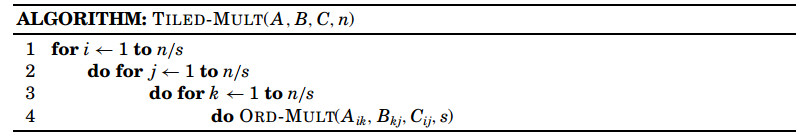
\includegraphics[width=\textwidth]{./Figures/Project2a/TiledMulti_Pseudo.jpg}
		\rule{35em}{0.5pt}
	\caption[Pseudocode for tiled multiplication]{
	Pseudocode for tiled multiplication.
	}
	\label{fig:TiledMulti_Pseudo}
\end{figure}
The idea is to base the size of the sub-matrices on the cache size and thereby utilize the cache in the best way (i.e. fewer cache faults).   

TMM is implemented by splitting the input matrices (A and B) into S sub-matrices in each dimension, then multiplying the sub-matrices producing the multiplied matrix (C). 
The value of S is calculated based on a value \verb!CACHE_SIZE_KB! which we choose depending on the platform. S is calculated so that three sub-matrices can fit in cache at the same time (as described in the article).
The calculation is as follows:
\begin{lstlisting}[numbers=left]
  ...
  // Needs to be 3 sub mats in cache at a time
  int allowedSizeOfSubMat = (CACHE_SIZE_KB*1024) / 3;
  int numOfSubMats = allowedSizeOfSubMat / sizeof(int);
  s = ceil( sqrt(numOfSubMats) );
  ... 
\end{lstlisting}
The multiplication of the sub-matrices is calculated with the naive matrix multiplication method. 
The biggest challenge in the implemtation was to seperate the input matrices int sub-matrices without actually creating new matrices, which would use a lot of extra memory and computation time. 
Instead we keep track of the start indices of the sub-matrices and just access A and B to get the values. 
To keep track of how far we have gotten in each direction in A and B and how big the next sub-matrices is, we maintain six variables:
\begin{lstlisting}[numbers=left]
  ...
  int subAnRows, subAnCols, subBnCols;
  int rowsVisitedA = 0;
  int colsVisitedA = 0;
  int colsVisitedB = 0;
  ...
\end{lstlisting}
The size of the new sub-matrix (e.g. \verb!subAnRows!) are updated each time we iterate in the corresponding direction (e.g. rows). 
The new value depends on how far we've gotten and the size of the input e.g.
\begin{lstlisting}
subAnRows = ceil( (double) (A->nRows - rowsVisitedA) / (double) (s - i) );
\end{lstlisting}

We only need three variables to maintain where we are in A, B and C, and not four, because of the constraint that A has to have as many coloumns as B has rows for the two to be multiplied. 
Maintaining these values also means that A and B can be multiplied without depending on that they are symmetric or have the same size, as long as they comply with forementioned constraint.



\section{Results and discussion}



\begin{figure}[htbp]
	\centering
		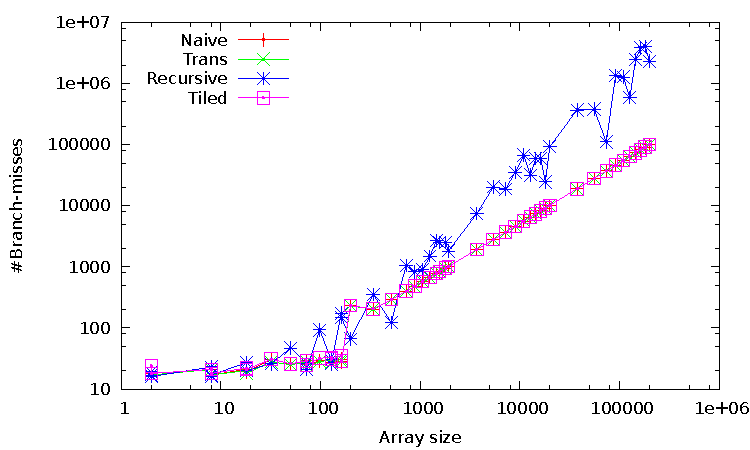
\includegraphics[width=\textwidth]{./Figures/Project2a/Branch_misses.pdf}
		\rule{35em}{0.5pt}
	\caption[Branch misses]{
	This shows how many branch misses we have for different sizes of arrays.
	}
	\label{fig:Branch_misses_p2a}
\end{figure}
We can see that the recursive function is above the others in branch miss predictions.
The reason is that for every calculation it has three choices.
That makes the branch miss predictions $ \Theta ((m\cdot n\cdot p)\cdot \frac{2}{3}) $.

\begin{figure}[htbp]
	\centering
		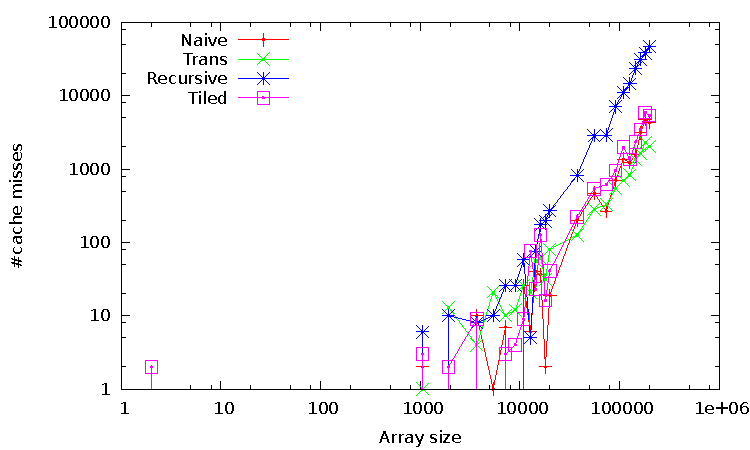
\includegraphics[width=\textwidth]{./Figures/Project2a/Cache_misses.pdf}
		\rule{35em}{0.5pt}
	\caption[Cache misses]{
	This shows the amount of cache misses we have for increasing sizes of arrays.
	}
	\label{fig:Cache_misses_p2a}
\end{figure}
This has a correlation with the graph for branch misses because if the recursive method has a lot og branch misses, then the system doesn't know what to load into the cache next time and thereby making a cache miss.


\begin{figure}[htbp]
	\centering
		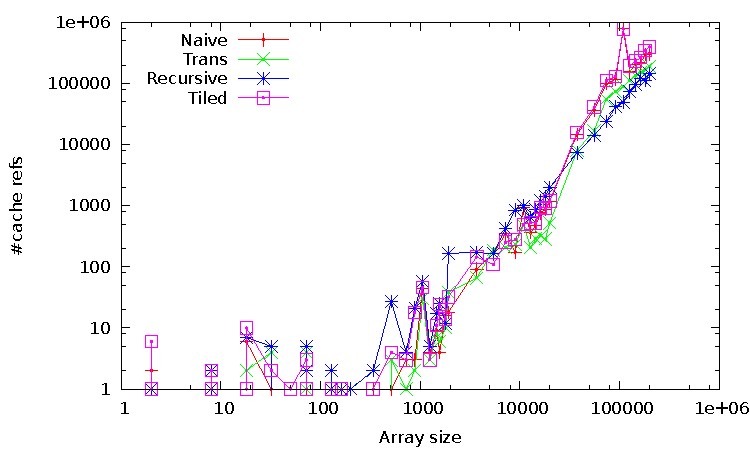
\includegraphics[width=\textwidth]{./Figures/Project2a/Cache_refs.pdf}
		\rule{35em}{0.5pt}
	\caption[Cache refs]{
	This shows the relation between array size and cache references.
	}
	\label{fig:Cache_refs_p2a}
\end{figure}
The naive and tiled algorithms make equally many references to the cache.
The Naive algorithm have to load a whole row for every calculation and the arrays are saved by columns which means it has to load the first element in every column.
The tiled is a little better but is still using a naive matrix multiplication after splitting the input matrix into smaller sub matrices.

\begin{figure}[htbp]
	\centering
		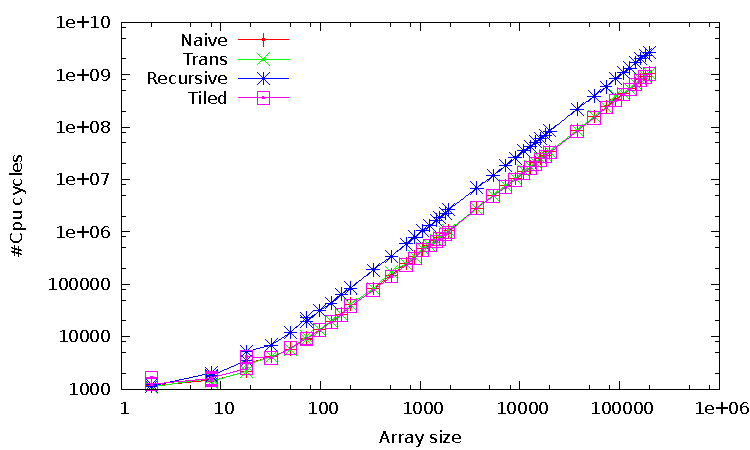
\includegraphics[width=\textwidth]{./Figures/Project2a/Cpu_cycles.pdf}
		\rule{35em}{0.5pt}
	\caption[CPU cycles]{
	
	}
	\label{fig:Cpu_cycles_p2a}
\end{figure}


\begin{figure}[htbp]
	\centering
		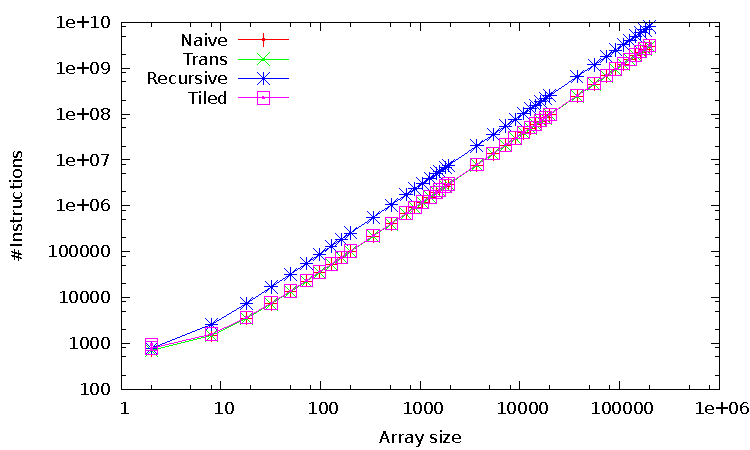
\includegraphics[width=\textwidth]{./Figures/Project2a/Instructions.pdf}
		\rule{35em}{0.5pt}
	\caption[Instructions]{
	Bla bla bla.
	}
	\label{fig:Instructions_p2a}
\end{figure}
